\documentclass[pdflatex,compress,mathserif]{beamer}

%\usetheme[dark,framenumber,totalframenumber]{ElektroITK}
\usetheme[darktitle,framenumber,totalframenumber]{ElektroITK}

\usepackage[utf8]{inputenc}
\usepackage[T1]{fontenc}
\usepackage{lmodern}
\usepackage[bahasai]{babel}
\usepackage{amsmath}
\usepackage{amsfonts}
\usepackage{amssymb}
\usepackage{graphicx}
\usepackage{multicol}

\newcommand*{\Scale}[2][4]{\scalebox{#1}{$#2$}}%

\title{PEMODELAN JARINGAN KOMUNIKASI}
\subtitle{Connectivity Troubleshooting}

\author{Tim Dosen Pengampu}

\begin{document}

\maketitle

\section{Basic Connectivity Troubleshooting}

\begin{frame}
	\frametitle{Ping}
	\begin{itemize}
		\item ICMP: Internet Control Message Protocol
		\begin{center}
			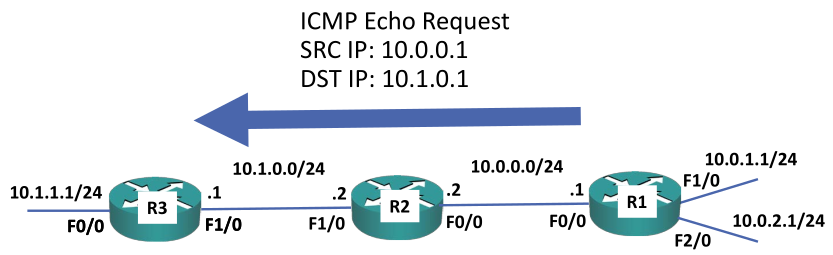
\includegraphics[width=\linewidth]{img/img01}
		\end{center}
	\end{itemize}
\end{frame}

\begin{frame}{Ping}
	\begin{itemize}
		\item ICMP: Internet Control Message Protocol
		\begin{center}
			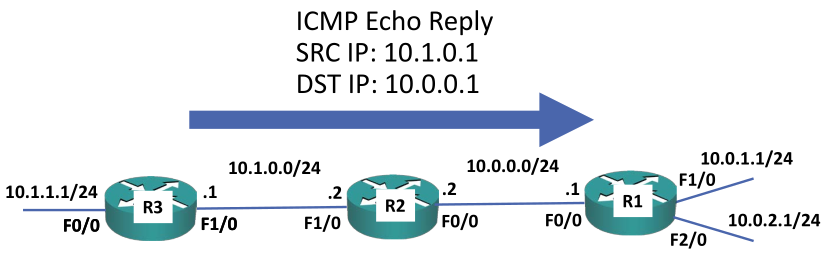
\includegraphics[width=\linewidth]{img/img02}
		\end{center}
	\end{itemize}
\end{frame}

\begin{frame}
	\frametitle{Ping Responses}
	\begin{itemize}
		\item If the ping is successful:
	\end{itemize}
	\texttt{R1\#ping 10.1.0.1
\\
		Type escape sequence to abort.
\\
		Sending 5, 100-byte ICMP Echos to 10.1.0.1, timeout is 2
 seconds:
\\
		.!!!!
\\
		Success rate is 80 percent (4/5), round-trip min/avg/max =
68/322/1076 ms} \\
\end{frame}

\begin{frame}{Ping Responses}
	\begin{itemize}
		\item If the router does not have a corresponding route or the destination IP
address does not respond:
	\end{itemize}
	\texttt{R1\#ping 172.16.1.1
\\
		Type escape sequence to abort.
\\
		Sending 5, 100-byte ICMP Echos to 172.16.1.1, timeout is 2
seconds:
\\
		.....
\\
		Success rate is 0 percent (0/5)} \\
\end{frame}

\begin{frame}{Ping Responses}
	\begin{itemize}
		\item If the router discards the packet (for example it is blocked by an Access
		Control List):
	\end{itemize}
	\texttt{R1\#ping 172.16.1.1
\\
		Type escape sequence to abort.
\\
		Sending 5, 100-byte ICMP Echos to 172.16.1.1, timeout is 2
seconds:
\\
		.....
\\
		Success rate is 0 percent (0/5)} \\
\end{frame}

\begin{frame}
	\frametitle{Extended Ping}
	\begin{itemize}
		\item Scenario: The user on PC1 complains that he can’t access services on PC3
		\item The problem is R4 does not have a route to 10.0.1.0/24
		\item Traffic which originates from a router always uses the IP address on the
outgoing interface as the source address
		\item A ping from R1 to 10.1.2.10 will succeed because R4 has a route to
10.0.0.1
	\end{itemize}
\end{frame}

\begin{frame}{Extended Ping}
	\begin{center}
		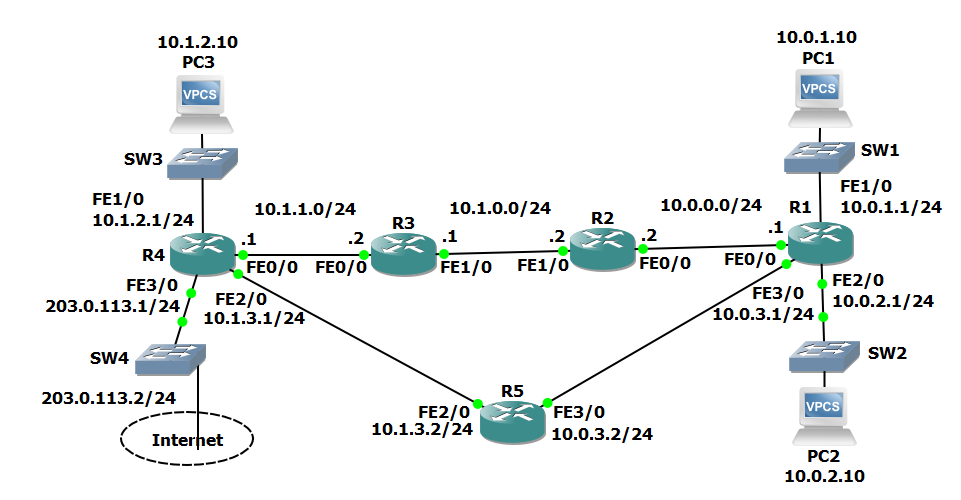
\includegraphics[width=\linewidth]{img/img03}
	\end{center}
\end{frame}

\begin{frame}{Extended Ping}
	\texttt{PC1> ping
10.1.2.10 \\
	10.1.2.10   icmp\_seq=1 timeout\\
	10.1.2.10   icmp\_seq=2 timeout\\
	10.1.2.10   icmp\_seq=3 timeout\\
	10.1.2.10   icmp\_seq=4 timeout\\
	10.1.2.10   icmp\_seq=5 timeout}\\
	\[ \]
	\texttt{R1\#ping 10.1.2.10
\\
	Type escape sequence to abort.
\\
	Sending 5, 100-byte ICMP Echos to 10.1.2.10, timeout is 2
seconds:
\\
	!!!!!}
\end{frame}

\begin{frame}{Extended Ping}
	\begin{center}
		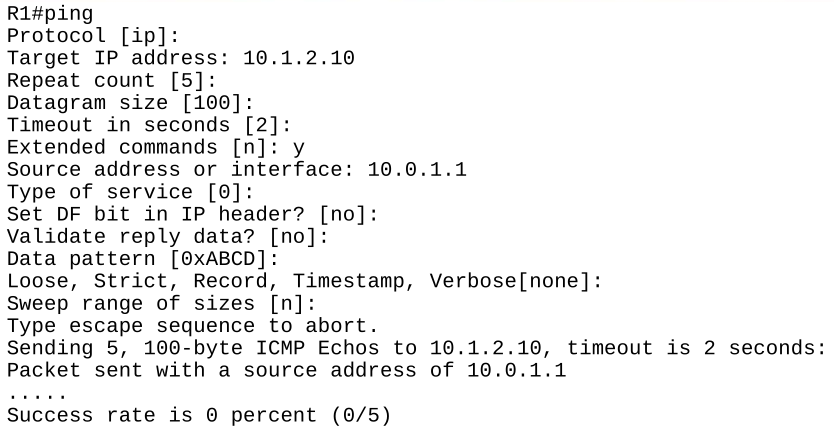
\includegraphics[width=\linewidth]{img/img04}
	\end{center}
\end{frame}

\begin{frame}
	\frametitle{Traceroute}
	\begin{center}
		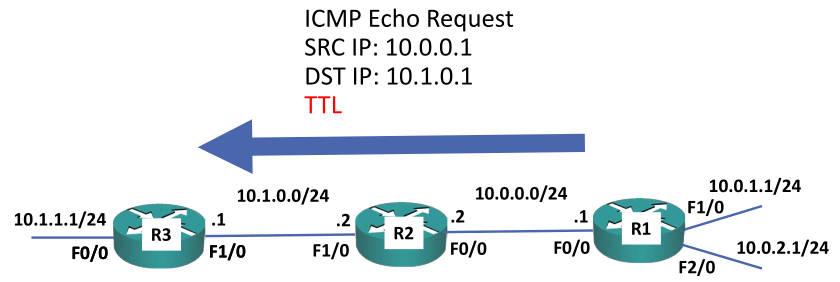
\includegraphics[width=\linewidth]{img/img05}
	\end{center}
\end{frame}

\begin{frame}{Traceroute}
	\begin{center}
		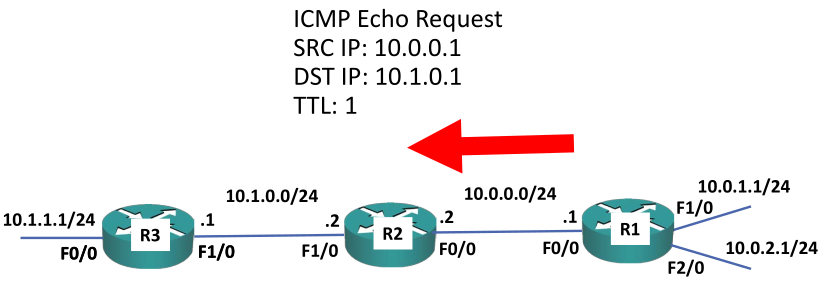
\includegraphics[width=\linewidth]{img/img06}
	\end{center}
\end{frame}

\begin{frame}{Traceroute}
	\begin{center}
		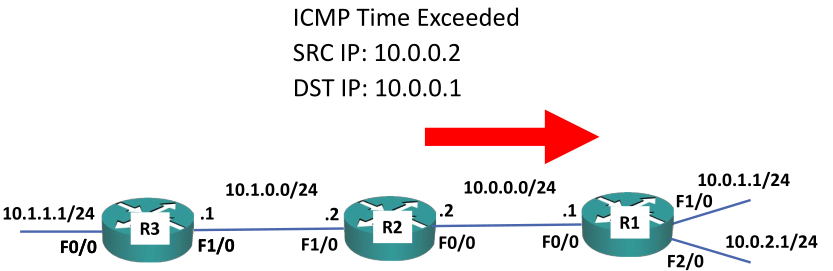
\includegraphics[width=\linewidth]{img/img07}
	\end{center}
\end{frame}

\begin{frame}{Traceroute}
	\begin{center}
		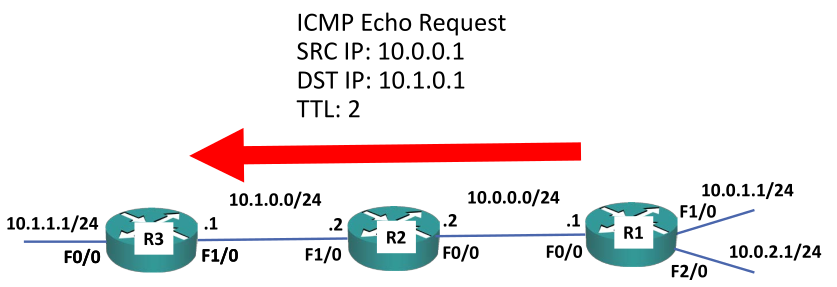
\includegraphics[width=\linewidth]{img/img08}
	\end{center}
\end{frame}

\begin{frame}{Traceroute}
	\begin{center}
		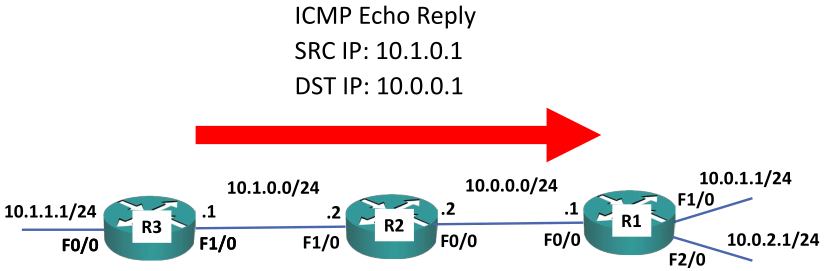
\includegraphics[width=\linewidth]{img/img09}
	\end{center}
\end{frame}

\begin{frame}
	\frametitle{Traceroute Responses}
	\begin{itemize}
		\item Successful Traceroute:
	\end{itemize}
	\begin{center}
		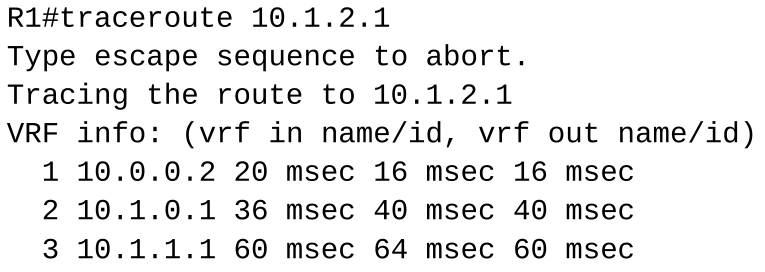
\includegraphics[width=\linewidth]{img/img10}
	\end{center}
\end{frame}

\begin{frame}{Traceroute Responses}
	\begin{itemize}
		\item The packet is getting as far as 10.1.0.1. Start troubleshooting there.
		\item Press Ctrl-Shift-6 to abort
	\end{itemize}
	\begin{center}
		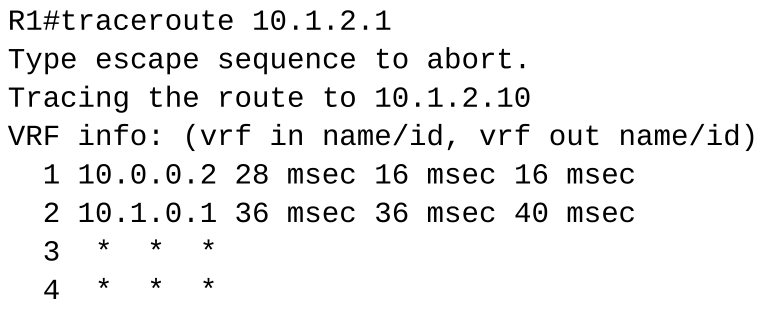
\includegraphics[width=\linewidth]{img/img11}
	\end{center}
\end{frame}

\begin{frame}
	\frametitle{Other Tools – Layer 1}
	\begin{itemize}
		\item Show ip interface brief
		\item Show interface
	\end{itemize}
\end{frame}

\begin{frame}
	\frametitle{Other Tools – Layer 2}
	\begin{itemize}
		\item Show arp
		\item Show mac address-table
	\end{itemize}
\end{frame}

\begin{frame}
	\frametitle{Other Tools – Layer 4}
	\begin{itemize}
		\item Telnet
	\end{itemize}
\end{frame}

\begin{frame}
	\frametitle{Other Tools – DNS}
	\begin{itemize}
		\item nslookup
		\item Ping by FQDN
	\end{itemize}
\end{frame}

\end{document}
